\section{Introduction}

% %% What is the problem?
% Utilizing large datasets for robotics -> GCRL from offline data
Developing controllers that can solve a range of tasks and generalize broadly in real-world settings is a long-standing challenge in robotics.
Such generalization in other domains such as computer vision and natural language processing has been attributed to training large machine learning models on massive datasets~\cite{krizhevsky2012imagenet}.
Consequently, one promising approach to robustly handle a wide variety of potential situations that a robot might encounter is to train on a large dataset of robot behaviors.
Prior work in robotics has demonstrated effectively generalization from training on large datasets for individual tasks, such as grasping~\cite{levine2017grasping, yu2021conservative}.
%%SL.3.1: It would be good to cite more non-conflicted papers, such as Lerrel's grasping paper, the Dieter Fox IRIS paper, and as many other relevant non-conflicted papers as you can find.
However, a general-purpose robot should be able to perform a wide range of skills, and should also be \textit{taskable}.
That is, it must be able to complete a specific task when specified by a human, including temporally extended tasks that require sequencing many skills together to complete.
This topic has been studied in prior work on goal-conditioned reinforcement learning, where a robot aims to perform a task given a desired end state~\cite{Khazatsky2021WhatCI, chebotar2021actionable, kalashnikov2021mtopt}.
%%SL.3.1: My suggestion: add many more citations, and also add "or other type of command~\cite{}" and add a bunch more citations. Don't skimp on citations, and definitely make sure to cite plenty of non-conflicted papers.
What remains to make these methods widely applicable for real-world robotics?
%%SL.3.1: It's good to pose questions, but it's not good to pose very open-ended questions, because this encourages lateral thinking (i.e., the reader will try to answer the question, and possibly not in the way that you expect). Perhaps a better organization would be to delete the above sentence and move the beginning of the next para (which explains the issues with GCRL) into the above para, and then start the next para by talking about the solution?
% Can the same approach, which has the benefit of requiring little human supervision, also be used to learn temporally extended tasks?

% % What is the problem? Long-horizon self-supervised RL OR Scaffolding long horizon policies
% % Scaffolding long horizon policies
% % Insight: (initial-state conditional) goal-conditioning allows you to compose subskills via planning
% % Insight: finetuning is required because 1. offline RL may not be perfect 2. there are errors from stitching skills together that must be corrected
% % Insight: planning can be a scaffold, but finetuning lets you train long-horizon goal-conditioned policies when you have the data
% % Online finetuning of long horizon policies via goal-conditioned planning
% A general purpose robot that is useful in unstructured environments must be able to perform a vast array of skills, and be \textit{taskable}.
% That is, it must be able to complete a specific task when specified by a human, including temporally extended tasks that require sequencing many skills together to complete.
% Deep reinforcement learning (RL) is a promising approach towards learning individual skills by optimizing a policy to maximize expected returns provided a reward function, and significant progress has been made on improving policy optimization.
% %%KF.2.26 Maybe it would be better to add 1-2 sentences to explain why GCRL is good for learning diverse tasks. I can think of several points, but Ashvin can probably summarize better:
% % - Configurable: Easy to specify tasks and rewards.
% % - Versatility: Can better share knowledge across different tasks of arbitrary horizons and efficiently reuse collected experiences.
% % - Compositionality: Goals can naturally serve as plans or curriculum in GCRL. 
% However, questions remain on how to apply deep RL in practice to train generalist robots that can accomplish useful tasks.
% One solution is self-supervised goal-conditioned RL, which learns general-purpose policies that aim to reach user-specified goal state.
% %%KF.2.26 The end of the first paragraph and the beginning of the 2nd paragraph are a bit disjointed. Maybe we could move the following sentences to the beginning of the 3rd paragraph instead.
% %%AVN.2.26 I see what you mean, we could potentially talk about how long horizon is a general case of GCRL here - I think we have to decide which flow to go with
% Prior work has showed how goal-conditioned RL utilizing prior data can learn taskable skills specified by a goal image without an external reward function~\cite{Khazatsky2021WhatCI}.
% %%SL.2.27: Maybe above sentence can be rephrased a bit more broadly, along the lines of something like: Prior work has studied varies methods for training goal-conditioned policies~\citep{lots_of_citations}, including [whatever]. [basically, include more than just one conflicted citation to acknowledge there is tons of research on this]
% This is accomplished by learning an affordance model on the offline trajectories that predicts potential goals in a scene, and offline RL to learn a policy from the same offline data.
% %%SL.2.27: The whole "affordance model" part is kind of coming out nowhere (not clear why it's important, necessary, or what it has to do with the preceding motivation)
% Can the same approach, which has the benefit of requiring little human supervision, be used to learn temporally extended tasks?
% % How can we learn to compose a set of skills from prior data?
% %%SL.2.27: Something in this logical chain feels missing -- I think it's the jump from "goal conditioned RL" to "temporally extended tasks". Perhaps another sentence is needed to "fill in the blank" about why temporally extended tasks are important? Basically something that just states but we really want temporally extended tasks, and these are hard (maybe the next para says this, but then the above sentence feels premature)

\begin{figure}[t!]
    \centering
    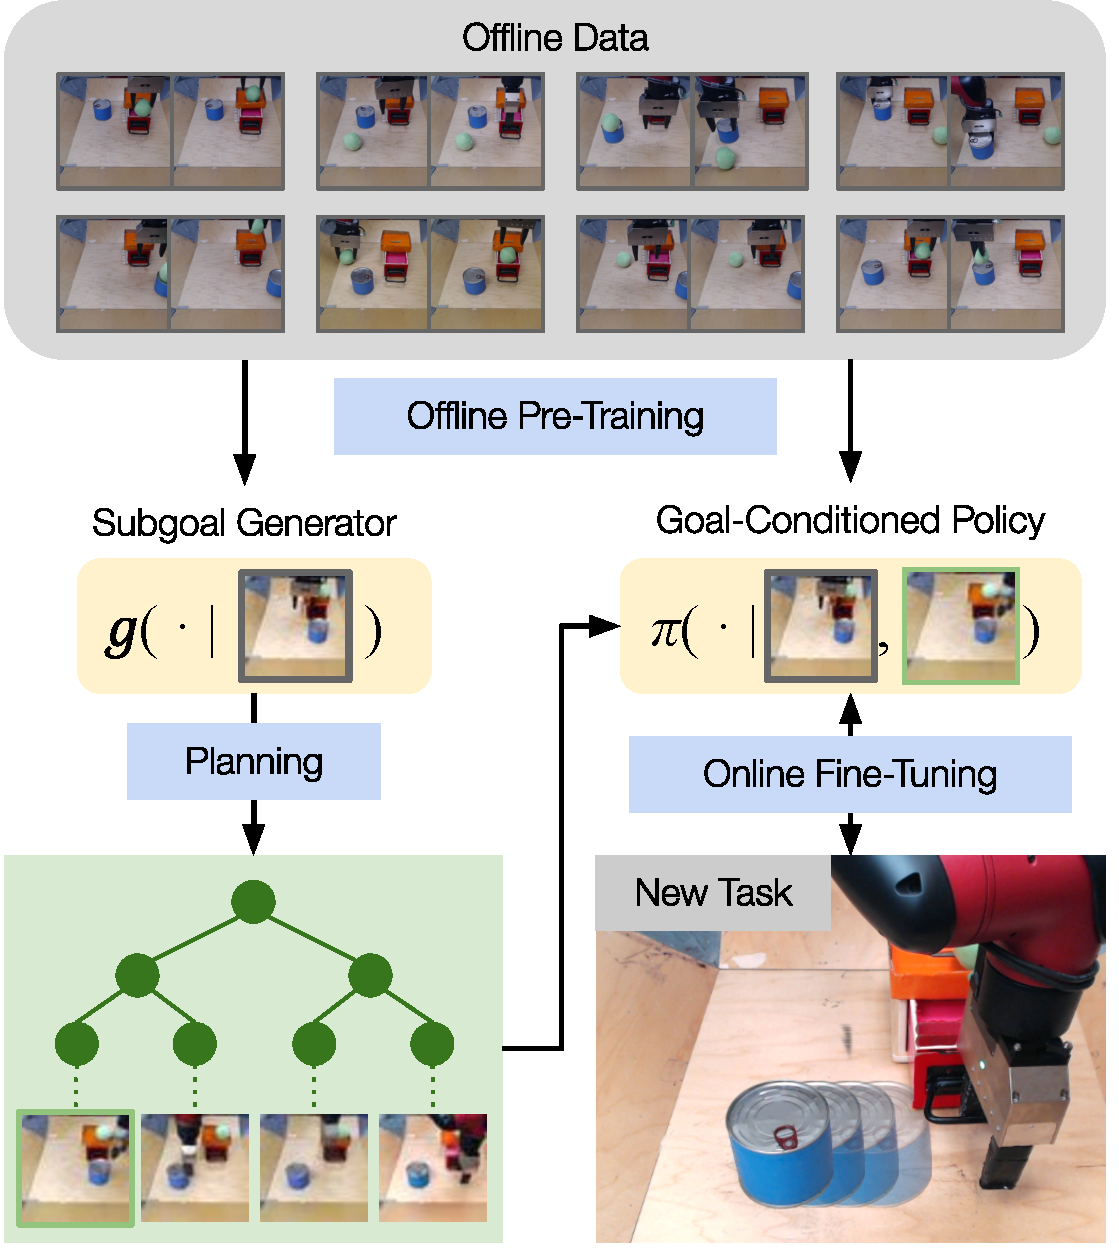
\includegraphics[width=.4\textwidth]{ptp/figures/intro.pdf}
    % \includegraphics[width=.4\textwidth]{example-image-a}
    % \vspace{-6mm}
    \caption{Our method, Plan to Practice (PTP), solves long-horizon goal-conditioned tasks by combining planning and fine-tuning.
    %%SL.3.1: See my comments before about planning having (usually) a pretty different meaning in robotics... without context, this is likely to lead to a misunderstanding.
    We begin with an offline dataset containing a variety of behaviors, and train a subgoal generator and goal-conditioned policy on this data. Then, to learn a more complex multi-stage tasks, we optimize over subgoals using the subgoal generator, which corresponds to a planning procedure over (visual) subgoals, and fine-tune the policy with online RL by practicing these subgoals. This enables the robot to solve multi-stage tasks directly from images.}
    %%SL.3.1: I edited the caption a fair bit. Generally, be careful not to inadvertently overclaim (variety of environments, new tasks, etc.). Readers will see right through it, and your credibility will be shot. Then they won't believe anything you say.
    \label{fig:intro}
    \vspace{-5mm}
\end{figure}

While goal-conditioned policies can be trained effectively for relatively short-horizon tasks, temporally extended multi-stage can pose a significant challenge for current methods. These tasks present a major exploration challenge during online learning, and a major challenge for credit assignment during offline learning.
%%SL.3.1: I edited the sentences below and replaced them with the one above. I edited the paragraphs below to better address exploration, but the "credit assignment" bit is a bit artificial, maybe there is a clearer term we can use that would fit with the next two paragraphs better? not sure...
%One challenge is in solving long-horizon, temporally extended tasks.
% Why is it interesting and important
%Goal-conditioned RL in theory can represent long horizon tasks as simply another task to generalize to.
%In practice, reinforcement learning with long-horizon tasks is known to be a difficult problem due to the challenges of exploration and credit assignment across a long time horizon.
%But unique challenges and opportunities appear in the context of goal-conditioned RL.
%%KF.2.26 Should we also talk about the challenges in terms of exploration and credit assignment across a long time horizon?
%%AVN yes, added above
%%SL.2.27: I'm actually confused by the above motivation: it says long-horizon is hard, but self-supervised (why?) goal-conditioned RL solves it. That feels like a non-sequitur -- we were saying before we want goal-conditioned, so if it just solves it, why do we need this paper? And in what sense is it self-supervised? Perhaps it would be cleaner to simply say that we want long-horizon goal-conditioned stuff [because of some reason], and this is hard, because while long-horizon RL is hard already, goal-conditioned long-horizon RL is even harder [with citations]
% While long-horizon tasks are in general more difficult, goal-conditioning offers the chance for composition.
% Training a long horizon policy without considering the sequencing of tasks
%%SL.2.27: what does that mean?
% may require an amount of data that is exponential in the length of the sequence.
%%SL.2.27: any RL problem may require an exponential amount of data, so this statement is largely meaningless
In this paper, we aim to address these challenges by combining two ideas. The first is that long-horizon goal-reaching tasks can be decomposed into shorter-horizon tasks consisting of subgoals. The second is that these subgoals can be used to \emph{fine-tune} a goal-conditioned policy online, even if its performance from offline data is poor.
% If we could compose skills together autonomously by sequentially setting coherent subgoals, the .
%%SL.2.27: Talking about sample efficiency here seems like a red herring, the issue is not just sample efficiency but being able to train policies that work at all.
% One idea that can be used to compose skills is conditional generative models of goals.
% Affordance models provide exactly this kind of knowledge: potential subgoals that can be reached from a given observation.
%%SL.2.27: reader doesn't know what an affordance model is at this point
The first idea enables us to address the exploration challenge, by automatically generating intermediate subgoals that can be ``practiced'' on the way to a longer-horizon final goal. In the framework of goal-conditioned RL, solving long-horizon tasks can be reduced to the problem of optimization over a sequence of subgoals for the goal-conditioned policy, and this optimization over subgoals can be regarded as a kind of high-level planning, where the optimizer selects waypoints for achieving a distant goal. The high-level planner itself can use a learned high-level model.

% This suggests that the key missing element is planning: by planning over future sequences, an agent can compose these kills.
% The plans can be provided to the lower level policy.
%%SL.2.27: As far as I can tell, the main idea in this paragraph is that the challenges of training long-horizon goal-conditioned policies can be overcome with [something]. But the [something] is not really explained (just the label "affordance model" is used without explanation). Perhaps it would be good to clearly and explicitly state the point (long-horizon + goal is hard, we can chain goals to make it easier), and try to more clearly define what "affordance" means (or use another more self-explanatory term)

%%KF.2.26 It might be better to motivate the utilization of offline data before talking about online fine-tuning?
%%AVN.2.26 I kind of quickly introduced offline data along with VAL above but maybe we need to expand on it more
However, if we rely entirely on offline data, credit assignment challenges make it difficult to perform longer-horizon tasks even with subgoal planning. Even if the offline RL policy performs well on each individual skill, there may be errors from stitching skills together because the initial states of each stage diverge from the offline data when they are composed together. In practice, this leads to poor performance when using only offline training. Therefore, the second key idea in our work is to utilize subgoal planning not merely to \emph{perform} a multi-stage task, but also to make it possible to \emph{practice} that task to finetune it online. While online training for temporally extended tasks is ordinarily difficult, by addressing the exploration challenge with subgoal planning, we make it possible for the robot to practice a series of relatively short-horizon tasks, which makes this kind of finetuning feasible. Thus, the planner acts both as a higher level policy when performing the task, and as a scaffolding curriculum for finetuning the lower-level goal-conditioned policy
%%SL.3.1: Rewrote the material below
%Composing subgoals in this manner from offline data, however, runs into the issue of distribution shift.
% With this kind of hierarchical approach, 
% there may be two issues.
%Especially if there are differences between the offline data and test environment, offline RL may not be perfect.
%%SL.2.27: Major disconnect here -- neither "hierarchical" nor "offline RL" were introduced before
%Even if the offline RL policy performs well on each individual skill, there may be errors from stitching skills together because the initial states of each stage diverge from the offline data when they are composed together.
%One solution to these problems of distribution shift is online fine-tuning.
By collecting data actively in a specific environment, we can directly experience the distribution shift and can use reinforcement learning to improve performance under this shift.
%Additionally, since the data that is collected is entire trajectories, this data can be used to fine-tune the long horizon goal-conditioned policy to actually solve the task directly.
%In this way, the planner can either act as a higher level policy to solve the task, or simply a scaffolding curriculum for the lower level goal-conditioned policy until the goal-conditioned policy can solve specific long-horizon tasks itself.
%%SL.2.27: Generally, I think this paragraph plays an important role: it serves to introduce the (highly nontrivial) idea that goal-conditioned + stitching multiple goals together by optimizing subgoals ("planning") can work very well if combined with offline RL and online finetuning. This is a subtle and extremely important idea. Right now the explanation though is pretty messy, maybe consider rewriting this paragraph, and make sure that any new concept (like offline RL) is introduced and there is a clear logical progression from the previous paragraph.

% Your approach
% Our technical contributions
To this end, we propose Planning to Practice (PTP), an approach that efficiently trains a goal-conditioned policy to solve
%%SL.2.24: It might be non-obvious in what sense the tasks are novel (and are they novel? if not, then maybe omit this part)
%%AVN.3.1 Took out "novel"
multi-step tasks by setting subgoals to exploit the compositional structure of the offline data.
%%SL.2.24: Hmm... so this presents the key idea as "exploiting the compositional structure of the offline data" -- is that really the key idea?
%%SL.2.27: same comment... not clear how the structure of the offline data is coming in; do you just mean that this is where affordances come from?
An outline is shown in Fig.~\ref{fig:intro}. Our approach is based around a planner that composes generated subgoals
% in the learned latent space
%%SL.2.27: what latent space?
%%AVN.3.1 we don't talk about latent spaces so far and its not that vital to the story so I'll just take it out
to guide the goal-conditioned policy during an online fine-tuning phase.
To propose diverse and reachable subgoals to form the candidate plans, we design a conditional subgoal generator based on conditional variational autoencoder (CVAE)~\cite{sohn2015cvae}.
Through training on the offline dataset, the conditional subgoal generator captures the distribution of reachable subgoals from a given state and generates sequences of subgoals from the learned latent space in a recursive manner.
%To efficiently find a feasible sequence of subgoals that leads to the desired goal state, we propose an efficient sampling-based planning algorithm using the conditional subgoal generator.
%%SL.3.1: commented out above sentence (it seems kind of uninformative at this level of detail, given that the reader won't have much context)
Our subgoal planning algorithm hierarchically searches for subgoals in a coarse-to-fine manner using multiple conditional subgoal generators that trained to generate goals at different temporal resolutions.
%We further devise a latent plan buffer that re-uses the previously selected plans as initial guesses in new episodes to enhance the chance of finding the plan.
%%SL.3.1: commented out the above (too low level, makes the method kind of come across as a bag of hacks)
Both the goal-conditioned policy and the conditional subgoal generators are pre-trained on the offline data, and the policy is fine-tuned on the novel target task. 
%%SL.2.24: Generally, this paragraph is reasonable, but a bit disorganized. I would recommend trying to structure it more top down, starting with the key ideas and subordinating the design choices under those key ideas.

% Summary of contributions
% Our experimental results.
%%SL.2.24: Maybe it would be better to have the first half of this paragraph clearly state the contributions of the work. This is especially important since it might not be entirely obvious to some readers what *precisely* is novel in the paper, so starting with a few sentences to explain the main contribution would remove this issue. If we can't clearly state the novel contribution in a few sentences here, it's likely the reviewers won't understand what the key contribution is either.
Our main contribution is a system for learning to solve long-horizon goal-reaching tasks by fine-tuning the goal-conditioned policy with subgoal planning in a learned latent space. 
We evaluate our approach on multi-stage robotic manipulation tasks with raw image observations and image goals in both simulation and the real world.
After being pre-trained on short demonstrations of primitive interactions, our approach is able to find feasible subgoal sequences as plans for unseen final goals by recursively generating subgoals with the learned conditional subgoal generators. By comparing our approach with both model-free methods and prior approaches that optimize over subgoals, we demonstrate that the produced plans significantly improve the learning efficiency and the resultant success rates during the online fine-tuning.
%%SL.3.1: This last sentence is pretty confusing to me: what is it exactly that we demonstrate? Can we try to state this more simply?

% Multi-task -> goals
% Deep reinforcement learning is a promising approach towards general robotics,  but the traditional deep RL paradigm optimizes a single known reward function. 
% For general-purpose robotics agents to operate in unstructured environments accomplishing useful tasks for humans, they must learn multiple skills and also be able to tasked to do any specific skill.
% This motivates the idea of self-supervised goal-conditioned reinforcement learning, which can be used to learn an array of skills that can be specified by a goal input.

% Paragraph 2 motivates goals -> planning & affordances; Paragraph 3 motivates offline data + finetuning as a way to use affordances. I think this will be a bit more logical, as the current organization kind of doesn't make it very clear why the offline data is an important part of the solution, making it instead feel a bit tacked-on.


% \section{Introduction}

% % Goal-conditioned RL
%     % - Enable robots to reach desired goal. This is important in many robotic applications.
%     % - Why this is hard? 
%     % - What we desire?
% Enabling the robot to solve goal-reaching tasks is a long-standing challenge in many robotic applications. Through reinforcement learning, we would like to learn goal-conditioned policy that controls the robot to strategically interact with the environment in the context of the current state and the desired goal~\cite{}. However, training such a policy from scratch would be extremely difficult for reaching distant goals in high-dimensional state spaces due to sparse rewards.  
% %%SL.2.24: My suggestion with this paragraph would be to start from a broader motivation about multi-task robots (like in the beginning of the abstract I suggested), and then motivate goals from there, rather than starting with goals as "first principles"

% % Utilizing offline data
%     % - Use offline data to tackle the problem.
%     % - Pre-training helps .
%     % - However, it is not enough.
%     % - As a result, it often does not work.
% Learning goal-conditioned policies can benefit from pre-training on offline data previously collected for the same or similar tasks before fine-tuning on the target task in an online manner~\cite{}. Such offline data is supposed to endow the policy with enough capability so that it can effectively explore the environment during online fine-tuning. In practice, however, na\"{i}vely pre-training and fine-tuning the policy can often lead to poor performance on the target task due to limitations of the offline data. First, the policy often only have access to insufficient amount of offline data so the under-trained policy can still struggle to collect additional useful data. Second, the policy needs to adapt to the distributional shift~\cite{} of the environment caused by different object arrangements or lighting conditions. Third, the pre-trained policy might not generalize to novel goals that are out of the distribution of the offline data. 
% %%SL.2.24: Somehow the argument for offline data comes across as a little incongruent to me. I think the issue is that it's not clear which problem the offline data is solving. Perhaps a better narrative structure (analogous to what I suggested in the abstract) might go something like this: Paragraph 1 motivates multi-task -> goals; Paragraph 2 motivates goals -> planning & affordances; Paragraph 3 motivates offline data + finetuning as a way to use affordances. I think this will be a bit more logical, as the current organization kind of doesn't make it very clear why the offline data is an important part of the solution, making it instead feel a bit tacked-on.

% % Utilizing the compositional structure
%     % - Recent advances 
%     % - Explain why this can help
%     % - Finding reasonable subgoals is not easy
%     % - Each state needs to be a valid state.
%     % - The transition between states needs to be possible
%     % - It forms a viable path from the initial state to the goal state
%     % - Existing works sample treat the samples as i.i.d
%     % - Although working for simple domains, ......
% To further facilitate reinforcement learning for reaching distant goals, several recent works aim to guide the goal-conditioned policy by planning a sequence of subgoals.
% %%SL.2.24: Generally, my suggestion would be to compartmentalize all references to prior work to one par tof the intro, somewhere in the beginning, whose goal is mainly to explain why the problem is hard (i.e., why prior work has not solved it before). But then don't keep referencing prior work in each paragraph, as this confuses the reader about what is new vs not new. Instead, thoroughly motivate and present the new things, and then relate them to prior work in the prior work section.
% The subgoals can break down the original long-horizon task into small snippets that are easier to solve. However, finding these subgoals can be very challenging in itself. In a reasonable plan, each subgoal needs to be a valid state sampled from the realistic state distribution in the first place. In addition, the sequence of subgoals is supposed to form a viable path that transits from the initial state to the desired goal state, \ie~the transition between adjacent subgoals in the plan needs to be feasible within a limited amount of time steps. Most existing works independently sample the subgoal of each step regardless of the initial state or the previously selected subgoals. Although these methods achieve performance improvements in simple domains, they often fall short in complicated robotic tasks with high-dimensional state spaces and large variations of initialization.
% %%SL.2.24: I think this paragraph also needs to be better tied to the central motivation -- it's not clear what problem is being solved with this or why it's needed. I think a good narrative structure might be to put this right after the motivation for goals (in the first paragraph), motivating it by explaining that training goal conditioned policies for goals that require multiple distinct steps (e.g., [example]) is very difficult (this is also kind of the structure I tried to follow in the abstract)


% % Our technical contributions
% To this end, we propose Planning to Practice (PTP), an approach that efficiently trains the goal-conditioned policy to solve novel
% %%SL.2.24: It might be non-obvious in what sense the tasks are novel (and are they novel? if not, then maybe omit this part)
% tasks by exploiting the compositional structure of the offline data.
% %%SL.2.24: Hmm... so this presents the key idea as "exploiting the compositional structure of the offline data" -- is that really the key idea?
% As shown in Fig.~\ref{fig:intro}, the key to our approach is a planner that composes generated subgoals in the learned latent space to guide the goal-conditioned policy during online fine-tuning. To propose diverse and reachable subgoals to form the candidate plans, we design a conditional subgoal generator based on conditional variational autoencoder (CVAE)~\cite{}. Through training on the offline dataset, the conditional subgoal generator captures the distribution of reachable subgoals from a given state and effectively generates sequences of subgoals from the learned latent space in a recursive manner. To efficiently find a feasible sequence of subgoals that leads to the desired goal state, we propose an efficient sampling-based planning algorithm using the conditional subgoal generator. Our algorithm hierarchically searches for subgoals in a coarse-to-fine manner using multiple conditional subgoal generators that trained to generate goals at different temporal resolutions. We further devise a latent plan buffer that re-uses the previously selected plans as initial guesses in new episodes to enhance the chance of finding the plan. Both the goal-conditioned policy and the conditional subgoal generators are pre-trained on the offline data and the policy is fine-tuned on the novel target task. 
% %%SL.2.24: Generally, this paragraph is reasonable, but a bit disorganized. I would recommend trying to structure it more top down, starting with the key ideas and subordinating the design choices under those key ideas.

% % Our experimental results.
% %%SL.2.24: Maybe it would be better to have the first half of this paragraph clearly state the contributions of the work. This is especially important since it might not be entirely obvious to some readers what *precisely* is novel in the paper, so starting with a few sentences to explain the main contribution would remove this issue. If we can't clearly state the novel contribution in a few sentences here, it's likely the reviewers won't understand what the key contribution is either.
% We evaluate our approach on multi-stage robotic manipulation tasks in both simulation and the real world. After being pre-trained on short demonstrations of primitive interactions, our approach is able to find the plan for novel goals across much longer time horizons by recursively generating subgoals with the learned conditional subgoal generators. By comparing our approach with model-free and planning-based
% %%SL.2.24: In general, be careful with use of the term "planning". Most roboticists will *not* think of what we're doing as planning. The mere fact that optimizing over subgoals for a goal-conditioned policy can be regarded as "planning" is actually rather radical, and while you could use that term, it definitely needs to be explained first (e.g., a sentence like this, perhaps in a prior paragraph: The optimization over subgoals based on the affordance model and the goal-conditioned policy can be regarded as a kind of high-level planning, where the optimizer selects ``waypoint'' images that can be used to provide a high-level scaffold for achieving a long-term goal. For example...)
% baselines, we demonstrate that the produced plans significantly improve the learning efficiency and the resultant success rates during the online fine-tuning. 



% \section{Introduction}

% % What is the problem? Long-horizon self-supervised RL OR Scaffolding long horizon policies
% % Scaffolding long horizon policies
% % Insight: (initial-state conditional) goal-conditioning allows you to compose subskills via planning
% % Insight: finetuning is required because 1. offline RL may not be perfect 2. there are errors from stitching skills together that must be corrected
% % Insight: planning can be a scaffold, but finetuning lets you train long-horizon goal-conditioned policies when you have the data
% % Online finetuning of long horizon policies via goal-conditioned planning
% A general purpose robot that is useful in unstructured environments must be able to perform a vast array of skills, and be \textit{taskable}.
% That is, it must be able to complete a specific task when specified by a human, including temporally extended tasks that require sequencing many skills together to complete.
% Deep reinforcement learning (RL) is a promising approach towards learning individual skills by optimizing a policy to maximize expected returns provided a reward function, and significant progress has been made on improving policy optimization.
% However, questions remain on how to apply deep RL in practice to train generalist robots that can accomplish useful tasks.
% This motivates the idea of self-supervised goal-conditioned RL, which can be used to learn an array of skills that can be specified by a goal input.
% Prior work has showed how goal-conditioned RL utilizing offline data can learn taskable skills specified by a goal image without an external reward function.
% Can the same approach, which has the benefit of requiring little human supervision, be used to learn temporally extended skills?
% % How can we learn to compose a set of skills from prior data?

% % Why is it interesting and important
% Reinforcement learning with long-horizon tasks is known to be a difficult problem, but unique challenges appear in the context of self-supervised goal-conditioned RL.
% We can conceive of a long horizon task as simply as another task to generalize to; ie. the goal conditioned policy can handle this if trained well.
% However, we should not need long sequences of skills to train this policy: this would require data that is exponential in the length of the sequence.
% Instead, we should able to compose skills together autonomously.
% This suggests that the key missing element is planning: by planning over future sequences, an agent can compose these kills.
% The plans can be provided to the lower level policy.

% With this approach, there may be two issues. First, offline RL may not be perfect, especially if there are differences between the offline data and test environment. Second, even if the offline RL policy performs well on each individual task, there may be errors from stitching skills together that can be corrected. This suggests that online fine-tuning may be useful in this setting. When fine-tuning, we actually collect data for the specific task we care about. So this data can actually be used to fine-tune the long horizon goal-conditioned policy to actually solve the task directly.

% % Your approach
% % Our technical contributions
% To this end, we propose Planning to Practice (PTP), an approach that efficiently trains the goal-conditioned policy to solve novel
% %%SL.2.24: It might be non-obvious in what sense the tasks are novel (and are they novel? if not, then maybe omit this part)
% tasks by exploiting the compositional structure of the offline data.
% %%SL.2.24: Hmm... so this presents the key idea as "exploiting the compositional structure of the offline data" -- is that really the key idea?
% As shown in Fig.~\ref{fig:intro}, the key to our approach is a planner that composes generated subgoals in the learned latent space to guide the goal-conditioned policy during online fine-tuning. To propose diverse and reachable subgoals to form the candidate plans, we design a conditional subgoal generator based on conditional variational autoencoder (CVAE)~\cite{}. Through training on the offline dataset, the conditional subgoal generator captures the distribution of reachable subgoals from a given state and effectively generates sequences of subgoals from the learned latent space in a recursive manner. To efficiently find a feasible sequence of subgoals that leads to the desired goal state, we propose an efficient sampling-based planning algorithm using the conditional subgoal generator. Our algorithm hierarchically searches for subgoals in a coarse-to-fine manner using multiple conditional subgoal generators that trained to generate goals at different temporal resolutions. We further devise a latent plan buffer that re-uses the previously selected plans as initial guesses in new episodes to enhance the chance of finding the plan. Both the goal-conditioned policy and the conditional subgoal generators are pre-trained on the offline data and the policy is fine-tuned on the novel target task. 
% %%SL.2.24: Generally, this paragraph is reasonable, but a bit disorganized. I would recommend trying to structure it more top down, starting with the key ideas and subordinating the design choices under those key ideas.

% % Summary of contributions

% % Multi-task -> goals
% % Deep reinforcement learning is a promising approach towards general robotics,  but the traditional deep RL paradigm optimizes a single known reward function. 
% % For general-purpose robotics agents to operate in unstructured environments accomplishing useful tasks for humans, they must learn multiple skills and also be able to tasked to do any specific skill.
% % This motivates the idea of self-supervised goal-conditioned reinforcement learning, which can be used to learn an array of skills that can be specified by a goal input.

% % Paragraph 2 motivates goals -> planning & affordances; Paragraph 3 motivates offline data + finetuning as a way to use affordances. I think this will be a bit more logical, as the current organization kind of doesn't make it very clear why the offline data is an important part of the solution, making it instead feel a bit tacked-on.
